\chapter{Leistung}
\begin{itemize}
    \item \underline{Wirkleistung $P$} \\
    Tatsächlich umgesetzte Energie in Watt [W]
    \item \underline{Blindleistung $Q$} \\
    Unerwünschte bzw. nicht nutzbare Energie in Volt-Ampere Relativ [var]
    \item \underline{Scheinleistung $S$} \\
    Gesamtleistung in Volt-Ampere [VA]
\end{itemize}

\section{Leistung bei Gleichstrom}
Allgemein gilt:

\begin{align}
    P&=U\cdot I \\
    P&=\frac{U^2}{R} \\
    P&=I^2\cdot R    
\end{align}

\begin{itemize}
    \item $P$ ... Leistung
    \item $U$ ... Spannung
    \item $I$ ... Strom
    \item $R$ ... Widerstand
\end{itemize}

\newpage

\subsection{Wirkleistung $P$}
\begin{align}
    P = U_w \cdot I = U \cdot I \cdot cos(\varphi)
\end{align}
\begin{itemize}
    \item $P$ ... Wirkleistung in [$W$]
    \item $U_w$ ... Wirkkomponente der Spannung in [$V$]
\end{itemize}

\subsection{Blindleistung $Q$}
\begin{align}
    Q = U_b \cdot I = U \cdot I \cdot sin(\varphi)
\end{align}
\begin{itemize}
    \item $Q$ ... Blindleistung in [$var$]
    \item $U_b$ ... Blindkomponente der Spannung in [$V$]
\end{itemize}
Die \textbf{induktive} Blindleistung ist \textbf{positiv}: $sin(\varphi) > 0 \rightarrow Q_L > 0$ \\
Die \textbf{kapazitive} Blindleistung ist \textbf{negativ}: $sin(\varphi) < 0 \rightarrow Q_C < 0$ \\

\subsection{Scheinleistung $S$}
\begin{align}
    S = U \cdot I
\end{align}
\begin{itemize}
    \item $S$ ... Scheinleistung in [$VA$]
\end{itemize}

\newpage

\section{Leistung bei Wechselstrom}
Bei einem sinusförmigen Verlauf der Spannung $u$ und des Stroms $i$ gelten folgende Gleichungen:
\begin{align}
    u = \hat{U} \cdot sin(\omega \cdot t) \hspace{1cm} i = \hat{I} \cdot sin(\omega \cdot t - \varphi)
\end{align}
Werden die Momentanwerte von $u$ und $i$ miteinander multipliziert, erhält man den Momentanwert der Leistung $p$:
\begin{align}
    p = u \cdot i = \hat{U} \cdot sin(\omega \cdot t) \cdot \hat{I} \cdot sin(\omega \cdot t - \varphi)
\end{align}
oder:
\begin{align}
    p = U_{eff} \cdot I_{eff} \cdot cos(\varphi) - U_{eff} \cdot I_{eff} \cdot (2\cdot \omega \cdot t - \varphi)
\end{align}

\begin{itemize}
    \item $p$ ... Momentanwert der Wechselstromleistung in [$W$]
    \item $U$ ... Effektivwert der Spannung in [$V$]
    \item $I$ ... Effektivwert des Stromes in [$A$]
\end{itemize}

\subsection{Leistungsfaktor}
Der Leistungsfaktor $cos(\varphi)$ gibt an, welchen Anteil die Wirkleistung an der Scheinleistung hat. Er erreicht bei ohmschen Lasten den maximalen Wert $1$:
\begin{align}
    P &= U \cdot I \cdot cos(\varphi) = S \cdot cos(\varphi) \\
    cos(\varphi) &= \frac{P}{S} 
\end{align}
\begin{itemize}
    \item $P$ ... Wirkleistung in [$W$]
    \item $S$ ... Scheinleistung in [$VA$]
    \item $cos(\varphi)$ ... Leistungsfaktor
\end{itemize}

\subsection{Kompensation}
\textit{GdE2 S.102} \\
Ein ohmsch-induktiver Verbraucher, wie z.B. ein Elektromotor, entnimmt dem Netz nicht nur Wirkleistung, sondern zum Aufbau des Magnetfeldes auch induktive Blindleistung. Der fließende Blindstromanteil belastet das Netz mit unerwünschten Spannungsabfällen und erhöhten Übertragungsverlusten. Ein parallel zum Verbraucher liegender Kondensator kompensiert die aus dem Netz bezogene Blindleistung und verbessert den Leistungsfaktor. Da die zugeführte Wirkleistung unverändert bleibt, ergibt sich folgendes Leistungsdreieck:

\begin{center}
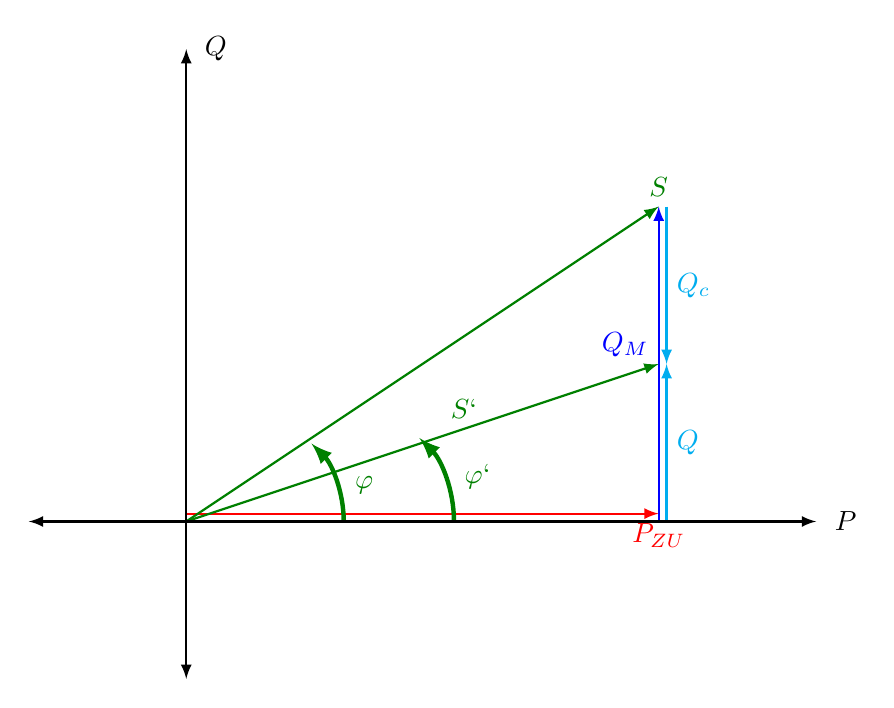
\begin{tikzpicture}[>=latex, scale = 2]
    \draw[style=help lines] (0,0) (3,2);

    \coordinate (pointer0) at (45:3);

    \coordinate (posX) at (0:4);
    \coordinate (posY) at (90:3);
    \coordinate (negX) at (180:1);
    \coordinate (negY) at (270:1);

    % \draw[->,thick,Green] (0,0) -- (pointer0) node[right, xshift=3pt, Green] {$S$};
    \draw[->,thick,red] (0,0.05) -- (3,0.05) node[below,  red] {$P_{ZU}$};
    
    \draw[->,thick,cyan] (3.05,0) -- (3.05,1) node[right, midway, cyan] {$Q$};
    \draw[->,thick,cyan] (3.05,2) -- (3.05,1) node[right, midway, cyan] {$Q_c$};
    \draw[->,thick,blue] (3,0) -- (3,2) node[left, midway,yshift = 7pt, blue] {$Q_M$};

    \draw[->,thick,green!50!black] (0,0) -- (3,2) node[above, green!50!black] {$S$};
    \draw[->,thick,green!50!black] (0,0) -- (3,1) node[above,midway,yshift = 5pt,xshift = 15pt, green!50!black] {$S`$};

    \draw[ultra thick, ->,green!50!black] (1,0) arc (0:45:0.7)node[right, midway,xshift = 3pt,yshift = -2pt ,green!50!black]{$\varphi$};
    \draw[ultra thick, ->,green!50!black] (1.7,0) arc (0:45:0.75)node[right, midway,xshift = 3pt,yshift = 0pt ,green!50!black]{$\varphi`$};
    

    \draw[->,thick,black] (0,0) -- (posX) node[right,xshift=3pt] {$P$};
    \draw[->,thick,black] (0,0) -- (posY) node[right,xshift=3pt] {$Q$};
    \draw[->,thick,black] (0,0) -- (negX);
    \draw[->,thick,black] (0,0) -- (negY);
\end{tikzpicture}
\end{center}

Wird der Leistungsfaktor von $cos(\varphi)$ auf $cos(\varphi')$ verbessert, folgt aus dem Leistungsdreieck mit der Blindleistung $Q_M$ des Verbrauchers und der Blindleistung $Q$ des Netzes die erforderliche Blindleistung $Q_C$:
\begin{align}
    Q_C = Q - Q_M
    \hspace{1cm}
    Q = P_{ZU} \cdot tan(\varphi')
    \hspace{1cm}
    Q_M = P_{ZU} \cdot tan(\varphi) \\
    \Rightarrow Q_C = P_{ZU} \cdot (tan(\varphi') - tan(\varphi))
\end{align}

\begin{itemize}
    \item $Q_C$ ... Blindleistung des Kondensators in [$var$]
    \item $P_{ZU}$ ... Wirkleistung des Verbrauchers in [$W$]
    \item $\varphi$ ... Phasenwinkel ohne Kompensation in [$\degree$]
    \item $\varphi'$ ... Phasenwinkel mit Kompensation in [$\degree$]
\end{itemize}

\begin{center}
\begin{tikzpicture}[>=latex, scale = 2]
    \draw[style=help lines] (0,0) (3,2);

    \coordinate (pointer0) at (45:3);

    \coordinate (posX) at (0:4.5);
    \coordinate (posY) at (90:1);
    \coordinate (negX) at (180:1);
    \coordinate (negY) at (270:3);


    \draw[->,thick,black] (0,0) -- (posX) node[right,xshift=3pt] {$+$};
    \draw[->,thick,black] (0,0) -- (posY) node[right,xshift=3pt] {$+j$};
    \draw[->,thick,black] (0,0) -- (negX);
    \draw[->,thick,black] (0,0) -- (negY);

    \draw[->,thick,red] (0,0.05) -- (3,0.05) node[right,yshift=7pt, red] {$I_w$};
    \draw[->,thick,red] (0,0) -- (3,-1) node[right, red] {$I`$};
    \draw[->,thick,red] (0,0) -- (3,-2.5) node[right,yshift = 7pt, red] {$I$};
    \draw[thick,red, dashed] (3,0.05) -- (3,-2.5) ;
    \draw[thick,cyan, ->] (3,0.05) -- (4,0.05) node[right,yshift = 7pt, cyan] {$U$};

    \draw[ultra thick, ->,green!50!black] (1,-0.8) arc (-45:45:0.6) node[right, midway,xshift = 3pt,yshift = -17pt ,green!50!black]{$\varphi$};
    \draw[ultra thick, ->,green!50!black] (1.8,-0.6) arc (-45:45:0.45) node[right, midway,xshift = 3pt,yshift = 0pt ,green!50!black]{$\varphi`$};
    
\end{tikzpicture}
\end{center}
    
\begin{center}
\begin{tikzpicture}[>=latex, scale = 2]
    \draw[style=help lines] (0,0) (3,2);

    \coordinate (pointer0) at (45:3);

    \coordinate (posX) at (0:4.5);
    \coordinate (posY) at (90:1.5);
    \coordinate (negX) at (180:1);
    \coordinate (negY) at (270:3);


    \draw[->,thick,black] (0,0) -- (posX) node[right,xshift=3pt] {$+$};
    \draw[->,thick,black] (0,0) -- (posY) node[right,xshift=3pt] {$+j$};
    \draw[->,thick,black] (0,0) -- (negX);
    \draw[->,thick,black] (0,0) -- (negY);

    \draw[->,thick,red] (0,0) -- (3,1) node[right, red] {$I`$};
    \draw[->,thick,red] (0,0.05) -- (3,0.05) node[right,yshift=7pt, red] {$I_w$};
    \draw[->,thick,red] (0,0) -- (3,-2.5) node[right,yshift = 7pt, red] {$I$};
    \draw[thick,red, dashed] (3,1) -- (3,-2.5) ;
    \draw[thick,cyan, ->] (3,0.05) -- (4,0.05) node[right,yshift = 7pt, cyan] {$U$};

    \draw[ultra thick, ->,green!50!black] (1,-0.8) arc (-45:45:0.6) node[right, midway,xshift = 3pt,yshift = -17pt ,green!50!black]{$\varphi$};
    \draw[ultra thick, ->,green!50!black] (1.8,0.6) arc (45:-45:0.4) node[right, midway,xshift = 3pt,yshift = 0pt ,green!50!black]{$\varphi`$};
    
\end{tikzpicture}
\end{center}